\documentclass[sigconf,nonacm]{acmart}

\begin{document}
\title{Chevrotain: A Conflict-free Replicated Data Type Key-Value Store}

\author{Alexandre Avreline}
\email{savrelin@students.cs.ubc.ca}
\affiliation{%
  \institution{Univeristy of British Columbia}
  \city{Vancouver}
  \state{British Columbia}
  \country{Canada}
}


\begin{abstract}
The abstract will be here
\end{abstract}


\begin{CCSXML}
<ccs2012>
   <concept>
       <concept_id>10011007.10010940.10010992.10010993.10010996</concept_id>
       <concept_desc>Software and its engineering~Consistency</concept_desc>
       <concept_significance>500</concept_significance>
       </concept>
   <concept>
       <concept_id>10003033.10003079.10011672</concept_id>
       <concept_desc>Networks~Network performance analysis</concept_desc>
       <concept_significance>500</concept_significance>
       </concept>
 </ccs2012>
\end{CCSXML}

\ccsdesc[500]{Networks~Network performance analysis}
\ccsdesc[500]{Software and its engineering~Consistency}

\ccsdesc[500]{Computer systems organization~Embedded systems}
\ccsdesc[300]{Computer systems organization~Redundancy}
\ccsdesc{Computer systems organization~Robotics}
\ccsdesc[100]{Networks~Network reliability}

\keywords{consistency, conflict-free replicated data types, key-value stores}

\maketitle

\section{Introduction}
Testing citation \cite{Davey:Lattices}
Testing referencing \ref{fig:sys}

\section{Background}

\subsection{State-Based Convergent Replicated Data Types (CvRDT)}

\subsection{Op-Based Commutative Replicated Data Types (CmRDT)}

\section{Design and Implementation}

\section{Evaluation}

\section{Related Work}

\section{Future Work}

\section{Conclusion}

\begin{figure}[h]
  \centering
  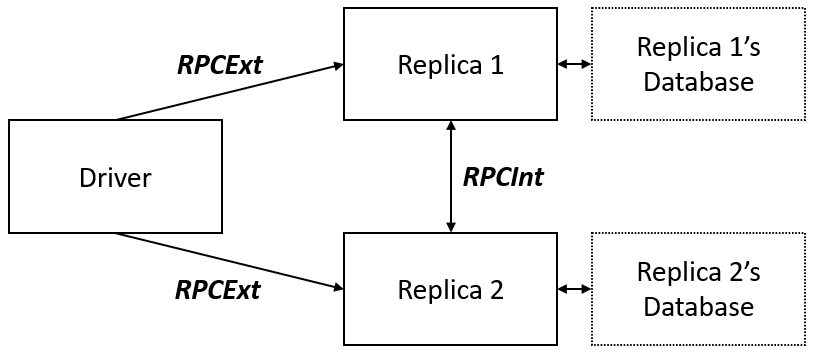
\includegraphics[width=7.5cm]{fig1}
  \caption{System Layout}
  \label{fig:sys}
\end{figure}

\bibliographystyle{ACM-Reference-Format}
\bibliography{report}

\end{document}
